\documentclass[11pt]{article}

\usepackage{acronym}
\usepackage[pdftex]{graphicx}
\usepackage{listings}
\usepackage{color}
\usepackage{paralist}
\usepackage[inline]{enumitem}
\usepackage[bookmarks]{hyperref}
\usepackage{bookmark}
\usepackage[capitalise,noabbrev]{cleveref}
\usepackage{hypernat}
\usepackage{url}

\usepackage[left=1in,right=1in,top=1in,bottom=1in]{geometry}
\usepackage[skip=11pt]{parskip}

\lstset{basicstyle=\ttfamily}

\setitemize{noitemsep,topsep=0pt,parsep=0pt,partopsep=0pt}
\setenumerate{noitemsep,topsep=0pt,parsep=0pt,partopsep=0pt}
\setdescription{noitemsep,topsep=0pt,parsep=0pt,partopsep=0pt}

%\newcommand{\TOOL}{\texttt{pate}}

\acrodef{DSL}{domain-specific language}
\acrodef{VM}{virtual machine}
\acrodef{SMT}{Satisfiability Modulo Theories}
\acrodef{IR}{intermediate representation}

\title{PATE Verifier User Manual (Version 0.9)}
\author{Galois (\href{mailto:pate-darpa-amp@galois.com}{pate-darpa-amp@galois.com})}

\begin{document}
\vspace*{-3cm}
{\let\newpage\relax\maketitle}

The PATE verifier is a static relational verifier for binaries with the
goal of proving that two binaries have the same observable behaviors.
It is intended for proving that security micropatches applied to
binaries are safe.  When it cannot, the verifier provides detailed
explanations that precisely characterize the difference in behavior
between the two binaries.  The verifier is intended to be usable by
\emph{domain experts}, rather than verification experts, and its
explanations are designed to be in domain terms as much as possible.
The verifier is intended to enable users to:
\begin{itemize}
\item precisely reason about the effects of patches applied to binaries,
\item explain potential differences in observable behaviors, accounting
  for all possible execution paths, and thus
\item reduce the time required to develop safe binary patches.
\end{itemize}

\vspace{0.25in}

\noindent\small{Distribution Statement A. Approved for public release: distribution unlimited.}


\newpage
\tableofcontents
\newpage

\acresetall

\section{Introduction}\label{sec:introduction}

This is the User Manual for the PATE verifier, updated to be consistent with the software release as of the end of AMP Phase 2 (7/28/23).
This manual can be found within the repository snapshot comprising the code release, in the directory \texttt{docs/usermanual}.
Much of the material in this document concerning how to build and run the verifier, as well as how to apply it to demonstration examples, can also be found within the repository.
In the sections below, we provide pathnames for the corresponding documentation files to be found in the software release.

Currently, the verifier supports PowerPC and AArch32 binaries (currently requiring statically linked ELF binaries).

The PATE verifier is a static relation verifier for binaries that builds assurance that micropatches have not had any adverse effects.
The verifier is a static relational verifier that attempts to prove that two binaries have the same observable behaviors.
When it cannot, the verifier provides detailed explanations that precisely characterize the difference in behavior between the two binaries.
The verifier is intended to be usable by \emph{domain experts}, rather than verification experts, and its explanations are designed to be in domain terms as much as possible.
After applying a micropatch to a binary, domain experts can apply the verifier to ensure that the effects are intended.

Note that while the verifier attempts to prove that the original and patched binaries have the same observable behaviors under all possible inputs, it is expected that they do not (or the patch would have had no effect).
When the two binaries can exhibit different behaviors, the verifier provides the user with an explanation of how and where the behavior is different.

If DWARF information is available in either the original or patched binary, the verifier will use that information to improve diagnostics.
Currently, function names, function argument names, local variable names, and global variable names can be used to make diagnostics more readable, for example, by replacing synthetic names with their source-level counterparts.
If working with binaries that do not come with DWARF debug information natively, see the \lstinline{dwarf-writer}\footnote{https://github.com/immunant/dwarf-writer} tool for a possible approach to adding DWARF debug information.

Note that recompiling a binary with a source patch applied can work for the purposes of the analysis, but can introduce complexities in cases where the compiler substantially rearranges code in response to the patch (which is common).
When the compiler re-arranges code, the verifier has a more difficult time aligning the code in the original and patched binaries, which can lead to confusing or unhelpful diagnostics.


\section{Building the PATE Verifier}
\label{sec:build-pate-verif}

The pate tool is written in Haskell and requires the GHC compiler
(version 8.6-8.10) and the cabal build tool to compile.  Building from
source can be accomplished as follows:
\begin{verbatim}
  git clone git@github.com:GaloisInc/pate.git
  cd pate
  git submodule update --init
  cp cabal.project.dist cabal.project
  cabal configure pkg:pate
  pate.sh --help
\end{verbatim}
The verifier also requires an SMT solver to be available in
``PATH``. The default is ``yices``, but ``z3`` and ``cvc4`` are also
supported.   The verifier can also be built as a Docker image:
\begin{verbatim}
  docker build . -t pate
\end{verbatim}
The correctness of the build can be confirmed by
\begin{verbatim}
docker run --rm -it -p 5000:5000 -v `pwd`/tests:/tests pate \
     --original /tests/aarch32/const-args.original.exe \
     --patched /tests/aarch32/const-args.patched.exe
\end{verbatim}


%%% Local Variables:
%%% mode: latex
%%% TeX-master: "user-manual"
%%% End:


\section{Invoking the \pate{} Verifier}
\label{sec:run-pate-verif}

Once \pate{} has been built as described in Section~\ref{sec:build-pate-verif}, use the docker container (or \texttt{pate.sh} script if building locally from source) to invoke \pate{}.

Invoking \pate{} via either docker or locally presents the user with an interactive terminal user interface for analyzing a pair of binaries.
Users provide at least the paths to two (the ``original'' and ``patched'') binaries at the command line when invoking \pate{}.
Additionally, we recommend also specifying the desired entry point, using \texttt{-s <symbol>}.
Providing the specific function of interest will enable \pate{} to begin reasoning closer to the relevant functionality of interest, greatly reducing the total analysis time required compared to starting from the program entry point.
Users may also wish to provide ``hint'' inputs that provide metadata mapping symbol names to addresses, easing analysis of stripped binaries.

The verifier accepts the following command line arguments:
\begin{verbatim}
  -h,--help                Show this help text
  -o,--original EXE        Original binary
  -p,--patched EXE         Patched binary
  -b,--blockinfo FILENAME  Block information relating binaries
  -s,--startsymbol ARG     Start analysis from the function with this symbol
  -d,--nodiscovery         Don't dynamically discover function pairs based on
                           calls.
  --solver ARG             The SMT solver to use to solve verification
                           conditions. One of CVC4, Yices, or Z3
                           (default: Yices)
  --goal-timeout ARG       The timeout for verifying individual goals in seconds
                           (default: 300)
  --heuristic-timeout ARG  The timeout for verifying heuristic goals in seconds
                           (default: 10)
  --original-anvill-hints ARG
                           Parse an Anvill specification for code discovery
                           hints
  --patched-anvill-hints ARG
                           Parse an Anvill specification for code discovery
                           hints
  --original-probabilistic-hints ARG
                           Parse a JSON file containing probabilistic function
                           name/address hints
  --patched-probabilistic-hints ARG
                           Parse a JSON file containing probabilistic function
                           name/address hints
  --original-csv-function-hints ARG
                           Parse a CSV file containing function name/address
                           hints
  --patched-csv-function-hints ARG
                           Parse a CSV file containing function name/address
                           hints
  --original-bsi-hints ARG Parse a JSON file containing function name/address
                           hints
  --patched-bsi-hints ARG  Parse a JSON file containing function name/address
                           hints
  --no-dwarf-hints         Do not extract metadata from the DWARF information in
                           the binaries
  -V,--verbosity ARG       The verbosity of logging output (default: Info)
  --save-macaw-cfgs DIR    Save macaw CFGs to the provided directory
  --solver-interaction-file FILE
                           Save interactions with the SMT solver during symbolic
                           execution to this file
  --proof-summary-json FILE
                           A file to save interesting proof results to in JSON
                           format
  --log-file FILE          A file to save debug logs to
  -e,--errormode ARG       Verifier error handling mode
                           (default: ThrowOnAnyFailure)
  -r,--rescopemode ARG     Variable rescoping failure handling mode
                           (default: ThrowOnEqRescopeFailure)
  --skip-unnamed-functions Skip analysis of functions without symbols
  --skip-divergent-control-flow
                           <DEPRECATED>
  --target-equiv-regs ARG  Compute an equivalence condition sufficient to
                           establish equality on the given registers after the
                           toplevel entrypoint returns. <DEPRECATED>
  --ignore-segments ARG    Skip segments (0-indexed) when loading ELF
  --json-toplevel          Run toplevel in JSON-output mode (interactive mode
                           only)
  --read-only-segments ARG Mark segments as read-only (0-indexed) when loading
                           ELF
  --script FILENAME        Save macaw CFGs to the provided directory
  --no-assume-stack-scope  Don't add additional assumptions about stack frame
                           scoping
  --ignore-warnings ARG    Don't raise any of the given warning types
\end{verbatim}


%%% Local Variables:
%%% mode: latex
%%% TeX-master: "user-manual"
%%% End:

\section{The PATE Terminal UI}
\label{sec:terminal-ui}

Once pate has been invoked at the command line (see Section~\ref{sec:run-pate-verif}), the user is presented with an interactive terminal user interface.

Internally, pate builds a tree representing the state of the analysis.
The interactive interface allows users to inspect the tree by selecting from a list of options based on the users current ``location'' in the tree.
The user makes a selection by entering a number representing the node of interest and hitting enter, or by entering a command.

\subsection{Example Usage}

After first starting pate, the user is presented with a list of entry points and makes a selection:
\begin{verbatim}
  Choose Entry Point
  0: Function Entry "_start" (segment1+0x435)
  1: Function Entry "parse_packet" (segment1+0x554)
  ?>
\end{verbatim}

The user enters \texttt{1}, selecting \texttt{parse\_packet}.
This starts pate's analysis at this point, and the user sees output of:

\begin{verbatim}
...........
0: Function Entry "parse_packet" (segment1+0x554) (User Request).........
1: segment1+0x580 [ via: "parse_packet" (segment1+0x554) ]
   (Widening Equivalence Domains).........
2: segment1+0x5ac [ via: "parse_packet" (segment1+0x554) ]
   (Widening Equivalence Domains)
3: Return "parse_packet" (segment1+0x554)
   (Widening Equivalence Domains)........
4: segment1+0x5cc [ via: "parse_packet" (segment1+0x554) ]
   (Widening Equivalence Domains).........
5: segment1+0x5e0 [ via: "parse_packet" (segment1+0x554) ]
   (Widening Equivalence Domains)........
6: segment1+0x600 [ via: "parse_packet" (segment1+0x554) ]
   (Widening Equivalence Domains)
7: Return "parse_packet" (segment1+0x554)
   (Widening Equivalence Domains).........
8: segment1+0x624 [ via: "parse_packet" (segment1+0x554) ]
   (Widening Equivalence Domains).........
Handle observable difference:
0: Emit warning and continue
1: Assert difference is infeasible (defer proof)
2: Assert difference is infeasible (prove immediately)
3: Assume difference is infeasible
4: Avoid difference with equivalence condition
?>
\end{verbatim}

Pate represents the analysis as a tree that can be navigated by the user.
The top level of the interactive process (reachable via the\texttt{top} command) is a list of all analysis steps that were taken, starting from the selected entry point.
Each pair of address and calling contexts defines a unique toplevel proof ``node.''
A given address and context may appear multiple times in the toplevel list, corresponding to each individual time that the address/context pair was analyzed.
The latest (highest-numbered) entry corresponds to the most recent analysis of an address/context.

Each entry point is associated with an equivalence domain: a set of locations (registers, stack slots and memory addresses) that are potentially not equal at this point.
Locations outside of this set have been proven to be equal (ignoring skipped functions).
The analysis takes the equivalence domain of an entry point and computes an equivalence domain for each possible exit point (according to the semantics of the block).

Here pate is asking how a detected observable difference should be handled.
The user selects \texttt{4} to capture the difference in the equivalence condition, and pate continues its analysis:

\begin{verbatim}
  0: Function Entry "parse_packet" (segment1+0x554) (User Request)
  1: segment1+0x580 [ via: "parse_packet" (segment1+0x554) ]
     (Widening Equivalence Domains)
  2: segment1+0x5ac [ via: "parse_packet" (segment1+0x554) ]
     (Widening Equivalence Domains)
  3: Return "parse_packet" (segment1+0x554)
     (Widening Equivalence Domains)
  4: segment1+0x5cc [ via: "parse_packet" (segment1+0x554) ]
     (Widening Equivalence Domains)
  5: segment1+0x5e0 [ via: "parse_packet" (segment1+0x554) ]
     (Widening Equivalence Domains)
  6: segment1+0x600 [ via: "parse_packet" (segment1+0x554) ]
     (Widening Equivalence Domains)
  7: Return "parse_packet" (segment1+0x554)
     (Widening Equivalence Domains)
  8: segment1+0x624 [ via: "parse_packet" (segment1+0x554) ]
     (Widening Equivalence Domains)
  9: segment1+0x644 [ via: "parse_packet" (segment1+0x554) ]
     (Widening Equivalence Domains)........
  10: segment1+0x644 [ via: "parse_packet" (segment1+0x554) ]
     (Re-checking Block Exits)........
  11: segment1+0x654 (original) vs. segment1+0x668 (patched)
     [ via: "parse_packet" (segment1+0x554) ]
     (Widening Equivalence Domains)........
  12: segment1+0x668 (original) vs. segment1+0x67c (patched)
     [ via: "parse_packet" (segment1+0x554) ]
     (Widening Equivalence Domains)
  13: Return "parse_packet" (segment1+0x554)
     (Widening Equivalence Domains)
  Continue verification?
  0: Finish and view final result
  1: Restart from entry point
  2: Handle pending refinements
  ?>
\end{verbatim}

The user selects \texttt{0} to finish and view the final result.

The pate analysis tree can be navigated by the user with \texttt{top} to move to the top of the tree, numbers to navigate ``into'' nodes, \texttt{up} to move ``up'' a node, and \texttt{ls} to redisplay the nodes available at a current level.

For example, to inspect the analysis results in the running example, the user may provide input as follows to view the equivalence condition:

\begin{verbatim}
  ...
  15: Final Result
  >15
  Final Result
  0: Assumed Equivalence Conditions
  1:   segment1+0x644 [ via: "parse_packet" (segment1+0x554) ]
  2: Binaries are conditionally, observably equivalent
  3: Toplevel Result
  >1
  segment1+0x644 [ via: "parse_packet" (segment1+0x554) ]
  0: ------
  1:   original
  2:   patched
  3: let -- segment1+0x684.. in not v40494
  >3
  let -- segment1+0x684
      v40487 = select (select cInitMemBytes@40467:a 0) 0x11045:[32]
      -- segment1+0x684
      v40490 = select (select cInitMemBytes@40344:a 0) 0x11044:[32]
      -- segment1+0x684
      v40494 = and (eq 0x80:[8] v40487) (not (eq v40490 (bvSum v40487 0x80:[8])))
   in not v40494
  0: With condition assumed
  1:   Event Trace: segment1+0x644 .. segment1+0x650 (original) vs.
       segment1+0x644 .. segment1+0x664 (patched)
  2: With negation assumed
  3:   Event Trace: segment1+0x644 .. segment1+0x650 (original) vs.
       segment1+0x644 .. segment1+0x664 (patched)
  >
\end{verbatim}

Continuing on, the user may view, for example, an example trace showing where the equivalence condition above does not hold:

\begin{verbatim}
  0: With condition assumed
  1:   Event Trace: segment1+0x644 .. segment1+0x650 (original) vs.
       segment1+0x644 .. segment1+0x664 (patched)
  2: With negation assumed
  3:   Event Trace: segment1+0x644 .. segment1+0x650 (original) vs.
       segment1+0x644 .. segment1+0x664 (patched)
  >3
  == Initial Original Registers ==
  pc <- 0x644:[32]
  r0 <- 0x0:[32]
  r1 <- 0x1:[32]
  r10 <- (3243, 0x0:[32])
  r11 <- (3342, 0x0:[32])
  r12 <- (2490, 0x0:[32])
  ...
  == Original sequence ==
  (segment1+0x644)
    Read 0x688:[32] -> 0x108:[32]
    r0 <- 0x108:[32]
  (segment1+0x648) r0 <- 0x758:[32]
  ...
  == Initial Patched Registers ==
  pc <- 0x644:[32]
  r0 <- 0x0:[32]
  r1 <- 0x1:[32]
  r10 <- (3243, 0x0:[32])
  r11 <- (3342, 0x0:[32])
  r12 <- (2490, 0x0:[32])
  ...
  == Patched sequence ==
  (segment1+0x644)
    Read 0x11044:[32] -> 0x80:[8]
    r1 <- 0x80:[32]
  (segment1+0x648)
    Read 0x11045:[32] -> 0x80:[8]
    r2 <- 0x80:[32]
\end{verbatim}

See the following subsections for details about how to interpret and interact with the terminal user interface.

\subsection{Status Indicators}

The \emph{prompt} indicates the status of the current node as follows:
\begin{itemize}
\item \texttt{*>} current node still has some active task running
\item \texttt{?>} current node requires user input
\item \texttt{!>} current node has raised a warning
\item \texttt{x>} current node has raised an error
\item \texttt{>} current node, and all sub-nodes, have finished processing
\end{itemize}

Similar to the prompt, nodes may be printed with a suffix that indicates some additional status as follows:
\begin{itemize}
\item \texttt{(*)} node still has some active task running
\item \texttt{(?)} node requires user input
\item \texttt{(!)} node has raised a warning
\item \texttt{(x)} node has raised an error
\end{itemize}
A status suffix indicates that the node, or some sub-node, has the given status.
e.g. at the toplevel the prompt \texttt{x>} indicates that an error was thrown during some block analysis, while the corresponding node for the block will have a \texttt{(x)} suffix.

\subsection{Navigation Commands}

\begin{itemize}
\item \texttt{\#} - navigate to a node, printing its contents
\item \texttt{up} - navigate up one tree level
\item \texttt{top} - navigate to the toplevel
\item \texttt{goto\_err} - navigate to the first leaf node with an error status
\item \texttt{next} - navigate to the highest-numbered node at the current level
\end{itemize}

\subsection{Diagnostic Commands}

\begin{itemize}
\item \texttt{status} - print the status of the current node
\item \texttt{full\_status} - print the status of the current node, without truncating the output
\item \texttt{ls} - print the list of nodes at the current level
\item \texttt{wait} - wait at the current level for more results. Exits when the node finishes, or
the user provides any input
\end{itemize}
When the prompt is \texttt{?>}, the verifier is waiting for input at some sub-node.
To select an option, simply navigate (i.e. by entering \texttt{\#}) to the desired choice.
For example, \texttt{goto\_prompt} - navigate to the first leaf node waiting for user input.


%%% Local Variables:
%%% mode: latex
%%% TeX-master: "user-manual"
%%% End:

% \section{Interacting with the Verifier}
\label{sec:repl}

Once the REPL (Read-EVAL-Print loop) has started, the first step of the analysis is to select an entry point to start from.
By default, the verifier starts verifying from the formal program entry point.
This is often not very useful (and can be problematic for complex binaries with a large \texttt{\_start} that causes problem for our code discovery).
Additionally, for changes with a known (or at least expected) scope of impact, analyzing just the affected functions is significantly faster.
To instead specify an analysis entry point, passing the \texttt{-s <function\_symbol>} option will start the analysis from the function corresponding to the given symbol.
Note that this requires function symbols to be provided for the binaries (either as embedded debug symbols or separately in one of the hint formats)::
\begin{verbatim}
  docker run --rm -it -v`pwd`/tests:/tests/hints pate \
             --original /tests/01.elf \
             --patched /tests/01.elf \
             --original-anvill-hints /tests/01.anvill.json \
             --patched-anvill-hints /tests/01.anvill.json \
             -s main
\end{verbatim}

The user can then select the desired entry point:
\begin{verbatim}
  Choose Entry Point
  0: Function Entry 0xdead
  1: Function Entry "my\_fun" (0xfeed)
  ?> 1
\end{verbatim}

The top level of the interactive process (reachable via the\texttt{top} command) is a list of all analysis steps that were taken, starting from the selected entry point.
Each pair of address and calling contexts defines a unique toplevel proof "node".
A given address and context may appear multiple times in the toplevel list, corresponding to each individual time that the address/context pair was analyzed.
The latest (highest-numbered) entry corresponds to the most recent analysis of an address/context.

Each entry point is associated with an equivalence domain: a set of locations (registers, stack slots and memory addresses) that are potentially not equal at this point.
Locations outside of this set have been proven to be equal (ignoring skipped functions).
The analysis takes the equivalence domain of an entry point and computes an equivalence domain for each possible exit point (according to the semantics of the block).

Differences between the two binaries may be reported into two ways:
\begin{itemize}
\item Observable trace differences -- library calls or writes to distinguished memory regions which have different contents or occur in different orders
\item Control flow divergence -- significant divergence in control flow between the programs (i.e. one program returns while the other calls a function)
\end{itemize}

% If we examine the first node (entering\texttt{1} at the prompt), we
% might see the following output:
% \begin{verbatim}
% Function Entry "my\_fun" (0xfeed)
% 0: Widening Equivalence Domains
% 1: Modify Proof Node
% 2: Predomain
% 3: Observably Equivalent
% 4: Block Exits
% 5:   Call to: "my\_sub\_fun" (0xdeef) Returns to: "my\_fun" (0xfeef)
% \end{verbatim}

% Element 5 indicates that, starting at the function entry
% for\texttt{my\_fun}, the original and patched
% binaries both necessarily call\texttt{my\_sub\_fun} next, returning to the
% address\texttt{0xfeef} within\texttt{my\_sub}.

For example, if a function \texttt{my\_fun} calls \texttt{my\_sub\_fun}, we might see the following toplevel output.
\begin{verbatim}
0: Function Entry "my\_fun" (0xfeed) (User Request)
1: Function Entry "my\_sub\_fun" (0xdeef) [ via: "my\_fun" (0xfeef) ]  (Widening Equivalence Domains)
2: 0xdeff [ via: "my\_sub\_fun" (0xdeef) <- "my\_fun" (0xfeed) ] (Widening Equivalence Domains)
4: Return "my\_sub\_fun" (0xdeef) (Widening Equivalence Domains)
5: 0xfeef [ via: "my\_sub\_fun" (0xdeef) <- "my\_fun" (0xfeed) ] (Widening Equivalence Domains)
6: Return "my\_fun" (0xfeed) (Widening Equivalence Domains)
\end{verbatim}
The contents of a node can be inspected by entering the corresponding number at the prompt.
A toplevel node contains sub-nodes corresponding to each possible "exit" that was discovered.
For example suppose we entered \texttt{2} at the prompt above.
The components of that node as displayed are:
\begin{itemize}
  \item\texttt{2:} - the number of this node, enter at the prompt to navigate to it and see a detailed view of the analysis step
\item\texttt{0xdeff} - the address that this analysis started from
\item \texttt{[ via: "my\_sub\_fun" (0xdeef) <- "my\_fun" (0xfeed) ]} -
    the calling context for this node, shown as the trace of function calls taken on the path to it (most recent call is first, left-to-right).
\item \texttt{(Widening Equivalence Domains)} - the reason this analysis step was taken. This is provided by whichever previous analysis step scheduled this node to be  processed.
\end{itemize}
The \emph{prompt} indicates the status of the current node as follows:
\begin{itemize}
\item \texttt{*>} current node still has some active task running
\item \texttt{?>} current node requires user input
\item \texttt{!>} current node has raised a warning
\item \texttt{x>} current node has raised an error
\item \texttt{>} current node, and all sub-nodes, have finished processing
\end{itemize}
Similar to the prompt, nodes may be printed with a suffix that indicates some additional status as follows:
\begin{itemize}
\item \texttt{(*)} node still has some active task running
\item \texttt{(?)} node requires user input
\item \texttt{(!)} node has raised a warning
\item \texttt{(x)} node has raised an error
\end{itemize}
A status suffix indicates that the node, or some sub-node, has the given status.
e.g. at the toplevel the prompt \texttt{x>} indicates that an error was thrown during some block analysis, while the corresponding node for the block will have a \texttt{(x)} suffix.

Navigation Commands:
\begin{itemize}
\item \texttt{\#} - navigate to a node, printing its contents
\item \texttt{up} - navigate up one tree level
\item \texttt{top} - navigate to the toplevel
\item \texttt{goto\_err} - navigate to the first leaf node with an error status
\item \texttt{next} - navigate to the highest-numbered node at the current level
\end{itemize}
Diagnostic Commands:
\begin{itemize}
\item \texttt{status} - print the status of the current node
\item \texttt{full\_status} - print the status of the current node, without truncating the output
\item \texttt{ls} - print the list of nodes at the current level
\item \texttt{wait} - wait at the current level for more results. Exits when the node finishes, or
the user provides any input
\end{itemize}
When the prompt is \texttt{?>}, the verifier is waiting for input at some sub-node.
To select an option, simply navigate (i.e. by entering \texttt{\#}) to the desired choice.
For example, \texttt{goto\_prompt} - navigate to the first leaf node waiting for user input.

% At the top level in the verifier's analysis data structure there is a
% list of block entry points that have been analyzed.  This includes:
% function entries, intermediate blocks within functions and function
% returns.

% Entry points may appear multiple times as a result of re-analysis due to
% additional equivalence information (i.e. propagating relaxed equivalence
% assumptions).

% Selecting an entry point will provide additional detail about its analysis.
% Most significantly a function call or intermediate block will provide a
% list of all possible exits, which can be individually inspected.


% Prompts
% -----

% Prompts are special proof nodes that affect the verifier behavior. After
% invoking\texttt{wait} (implicitly invoked after providing any prompt
% input), the verifier prints completed nodes as they are finished until
% it becomes blocked on a prompt. Once a prompt is available,\texttt{wait}
% implicitly navigates to it and presents the list of available choices.

% For example::
% \begin{verbatim}
%   Control flow desynchronization found at: GraphNode segment1+0x4114 [ via: "transport\_handler" (segment1+0x400c) ]
%   0: Choose synchronization points
%   1: Assert divergence is infeasible
%   2: Assume divergence is infeasible
%   3: Remove divergence in equivalence condition
%   4: Defer decision
%   ?>
% \end{verbatim}

% At this point the analysis is blocked, waiting for input before
% proceeding.  Normal navigation commands can be used here
% (\texttt{up},\texttt{top}, etc) to see the surrounding analysis context
% for this prompt.  However, navigating to any of these options
% (i.e. entering a number at this prompt) will take the corresponding
% action and resume the analysis.

% After input is provided for the prompt, the repl will implicitly
% navigate back to the toplevel and\texttt{wait}.

% Ad-hoc choices
% ----

% Some choices can be made ad-hoc, without blocking the analysis waiting
% for input. For example, most toplevel nodes have a\texttt{Modify Proof
%   Node} element, which presents a list of actions the user can request
% to perform on the given node. Any requested actions will occur after the
% current analysis step is finished, and often will then prompt the user
% for additional input.

%%% Local Variables:
%%% mode: latex
%%% TeX-master: "user-manual"
%%% End:
 % out of date - needs updating
% \section{Demonstration scenario}
\label{sec:demonstr-scen}

This section contains a detailed walk through of a demonstration of using the verifier to verify a patch to AMP Challenge 10.

From the repository root directory, run the verifier in its docker container:
\begin{verbatim}
  docker run --rm -it -v `pwd`/demos/may-2023/challenge10:/challenge10 pate \
             --original /challenge10/challenge10.original.exe \
             --patched /challenge10/challenge10.patched.exe \
             -b /challenge10/challenge10.toml \
             --original-bsi-hints /challenge10/challenge10.json \
             --patched-bsi-hints /challenge10/challenge10.json \
             --original-csv-function-hints /challenge10/challenge10.csv \
             --patched-csv-function-hints /challenge10/challenge10.csv \
             -s transport\_handler
\end{verbatim}

The file \texttt{challenge10.toml} specifies additional metadata needed for verification.
Specifically it instructs the verifier to start decoding the binary in thumb mode.

The file \texttt{challenge10.json} contains symbol information extracted using the BSI tool.
This information is used to identify functions that should use stub semantics rather than be analyzed (e.g. libc calls).

The file \texttt{challenge10.csv} contains manually-defined symbol information that was not automatically extracted from the BSI tool.
This is necessary to handle some PLT stubs that were not identified.

The last line tells the verifier to start the analysis at the function corresponding to the symbol \texttt{transport\_handler}, which is known from the BSI symbol data.
This is the function in which the patch appears.

Once the verifier starts printing output it can be interrupted at any time by pressing ENTER, but will continue processing in the background.
Its results can then be interactively inspected as they become available.

See Section~\ref{sec:repl}for more information on how to interact with the verifier's Read-Eval-Print loop.

\noindent\textbf{Step 1: Select the entry point and wait}

 Select \texttt{1} to start the analysis from the \texttt{transport\_handler} function.
\begin{verbatim}
  Choose Entry Point
  0: Function Entry segment1+0x3ba9
  1: Function Entry "transport\_handler" (segment1+0x400c)
  ?> 1
  ....................
  0: Function Entry "transport\_handler" (segment1+0x400c) (User Request) (!).
  ...
\end{verbatim}

 The verifier then proceeds to print out each analysis step until user input is required.

 \noindent\textbf{Step 2: Choose a synchronization point}

 \begin{figure}[ht]
  \centerline{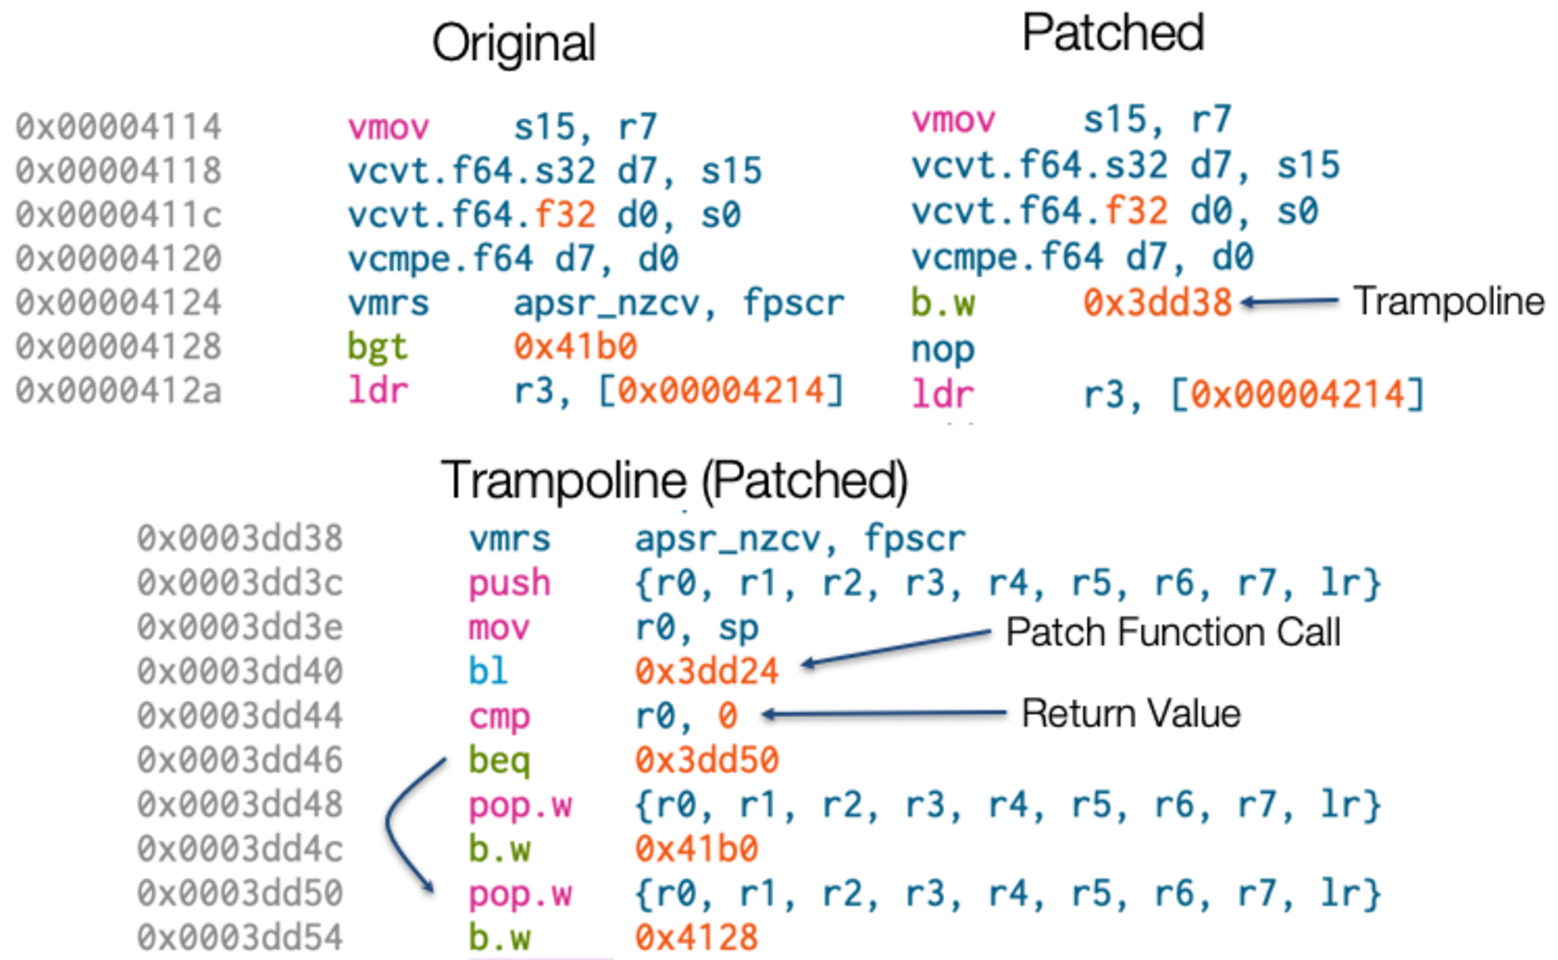
\includegraphics[width=0.9\linewidth]{patch.pdf}}
  \caption{Comparison of aligned regions in original and patched
    binaries for Challenge 10}
\label{fig:aligned}
\end{figure}

During the analysis of the block starting at \texttt{0x4114} the analysis encounters a control flow divergence.
This is an expected result of the patch, which, as shown in Figure~\ref{fig:aligned}, has inserted a trampoline starting at \texttt{0x4128}.
If the verifier is polling for output this will appear automatically, otherwise if the output was interrupted we can navigate to prompt by executing \texttt{top} followed by \texttt{goto\_prompt}:
\begin{verbatim}
  ?>goto\_prompt
  Control flow desynchronization found at: GraphNode segment1+0x4114
                   [ via: "transport\_handler" (segment1+0x400c) ]
  0: Ignore divergence (admit a non-total result)
  1: Assert divergence is infeasible
  2: Assume divergence is infeasible
  3: Remove divergence in equivalence condition
  4: Choose synchronization points
  5: Defer decision
  ?>
\end{verbatim}
Again, referring to Figure~\ref{fig:aligned} we can see where this happens in the code.
We can check the context of this choice by executing \texttt{up} then \texttt{up} to see the node that was being processed when this prompt was created.::
\begin{verbatim}
  ?>up
  ...
  ?>up
  segment1+0x4114 [ via: "transport\_handler" (segment1+0x400c) ] (Widening Equivalence Domains)
  0: Widening Equivalence Domains
  1: Modify Proof Node
  2: Predomain
  3: Observably Equivalent
  4: Block Exits (?)
  5:   Call to: "puts" (segment1+0x33ac) Returns to: "transport\_handler"
       (segment1+0x41b8) (original) vs. Call to: segment1+0x3dd24
      Returns to: "transport\_handler" (segment1+0x3dd44) (patched) (?)
  ?>
\end{verbatim}

Here we see that, from \texttt{0x4114} there are disagreeing block exits.
Specifically in the original program the block can exit with a call to \texttt{puts} while the patched function exits with a call to the anonymous function at \texttt{0x3dd24} (the inserted patch function).

To handle this, we need to instruct the verifier to perform a single-sided analysis on each program, and specify the point at which control flow re-synchronizes.
Specifically, we need to provide instruction addresses for the original and patched programs where, if execution reaches these addresses, both programs will resume in lockstep (i.e. all possible block exits (function calls) will be equal).
We navigate to the prompt with \texttt{goto\_prompt} and select \texttt{4: Choose synchronization points}.

We are then prompted to provide a pair of program points by selecting from a list of instructions.
With a separate analysis we can determine that the required synchronization points are \texttt{segment1+0x3dd44 (patched)} and \texttt{segment1+0x4128 (original)}.
As shown in Figure~\ref{fig:aligned}  at address \texttt{0x3dd44} (in the inserted trampoline), the patched program mirrors the branch instruction at \texttt{0x4128} in the original program.

Select these instructions from the list (one at a time) and the analysis will then continue.

\noindent\textbf{Step 3: Generate an equivalence condition}

The top-level nodes produced after this point are suffixed by \texttt{(original)} or \texttt{(patched)}, indicating which single-step analysis they correspond to.
After some analysis, the verifier prompts with another control flow desynchronization.
\begin{verbatim}
  Control flow desynchronization found at: GraphNode segment1+0x4128 (original) vs.
       segment1+0x3dd44 (patched) [ via: "transport\_handler" (segment1+0x400c) ]
  0: Ignore divergence (admit a non-total result)
  1: Assert divergence is infeasible
  2: Assume divergence is infeasible
  3: Remove divergence in equivalence condition
  4: Choose synchronization points
  5: Defer decision
  ?>
\end{verbatim}
This desynchronization indicates that control flow may still diverge between the original and patched programs after the synchronization point we provided.
This is exactly the intended result of our patch: after this point the program control flows \emph{may} be equal (i.e., in the case where the patch has simply recovered the original behavior of the program), but they may also be unequal (i.e., in the case where the patch has modified the program behavior).

Since this desynchronization precisely describes the non-equal branching behavior, we can exclude it from our analysis by asserting its negation as our generated *equivalence condition*.
This is option \texttt{3: Remove divergence in equivalence condition.}

After some analysis a similar prompt is given (corresponding to the inverse branching behavior), which we similarly handle by selecting \texttt{3} to assert the negation of this path condition.

The analysis then proceeds with this desynchronization omitted (and with a generated equivalence condition asserted at the synchronization point).

***********************************************************************

THIS IS THE POINT AT WHICH THE CURRENT DOCKER IMAGE (as of 7/27/23) throws an error.
So below here is not verified against actual execution.

***********************************************************************

\noindent\textbf{Step 4: Strengthening the equivalence domain}

After some time, the analysis eventually halts with a prompt indicating that a control flow difference has been found at \texttt{0x4181}.
With some investigation we can determine that this difference is spurious.
At the prompt, navigate to the toplevel node for \texttt{0x4181} via \texttt{up} then \texttt{up}, and select the option \texttt{2: Predomain}
\begin{verbatim}
  ?>up
  ..
  ?>up
  segment1+0x4181 [ via: "transport\_handler" (segment1+0x400c) ]
            (Widening Equivalence Domains)
  0: Widening Equivalence Domains
  1: Modify Proof Node
  2: Predomain
  3: Observably Equivalent
  4: Block Exits (?)
  5:   Call to: "err" (segment1+0x33ec) Returns to: "transport\_handler"
      (segment1+0x4191)
  6:   Call to: "err" (segment1+0x33ec) Returns to: "transport\_handler"
         (segment1+0x4191) (original) vs. Branch to: "transport\_handler"
         (segment1+0x402d) (patched) (?)
  ?>2
\end{verbatim}

The output here indicates that, although control flow is synchronized between the programs, several registers as well as global memory values are excluded from the equivalence domain (i.e., not known to be necessarily equivalence at this point).

The source of this inequivalence can be traced to the instruction immediately following the synchronization point at \texttt{0x412a} (\texttt{top} then \texttt{25} then \texttt{2}).
At this point, the equivalence domain has excluded \texttt{r0-r7} as well as the stack pointer and several stack slots.
This spurious inequivalence is a result of the trampoline saving and then restoring these registers onto the stack before resuming normal control flow.
The analysis has not retained enough context about the trampoline execution to automatically prove that this save/restore operation is sound.

We can instruct the verifier to strengthen the equivalence domain by explictly asserting that, at this program point, these registers are necessarily equivalent between the original and patched programs.
At the node for \texttt{0x412a} (\texttt{top} then \texttt{25}), select the option \texttt{1: Modify Proof Node}.
From this list we add an assertion by selecting \texttt{1: Assert condition}.

After providing this input, we are presented with the same control flow desynchronization prompt, which we now defer by selecting \texttt{4: Defer decision}, which will then present the prompt for the assertion we wish to add
\begin{verbatim}
  Include Register:
  0: r0
  1: r1
  2: r13
  3: r2
  4: r3
  5: r4
  6: r5
  7: r7
  8: Include Remaining Registers
  9: Exclude Remaining Registers
  ?> 8
\end{verbatim}

This is the list of registers that were excluded from the equivalence domain from \texttt{0x412a} Select \texttt{8} to include all of the given registers.
This choice results in an assertion that all of the user registers are necessarily equal between the original and patched programs when they both reach \texttt{0x412a}.
The analysis then proceeds by propagating the assertion up several nodes (indicated by the \texttt{Propagating Conditions} status), which is then eventually discharged.
The subsequent proof nodes are then re-checked under this new assertion, and correspondingly strengthened equivalence domain.

\noindent\textbf{Step 5: Propagating and interpreting the equivalence condition}

The verifier can now complete the analysis, prioviding a proof that the programs are exactly equivalent under the generated equivalence condition.
By default the condition is only asserted at exactly the location it is needed, however it can also be propagated to the entry point, in order to compute a sufficient condition at the beginning of the function call.

To do this, we navigate to the synchronization node (\texttt{top} then \texttt{57}) where we can see that an equivalence condition has been assumed.
However this is only in terms of the condition registers at this point.
Select \texttt{1: Modify Proof Node} and then \texttt{21:   Propagate fully}.

Then select \texttt{2: Handle pending refinements} at the next prompt to handle the requested action.
Once finished, the resulting equivalence condition can be examined by navigating to the node corresponding to the function entry point for \texttt{transport\_handler}.

%%% Local Variables:
%%% mode: latex
%%% TeX-master: "user-manual"
%%% End:
 % out of date - needs updating
\clearpage
\section{Acknowledgement}

This material is based upon work supported by the Defense Advanced
Research Projects Agency (DARPA) and Naval Information Warfare Center
Pacific (NIWC Pacific) under Contract Number N66001-20-C-4027. Any
opinions, findings and conclusions or recommendations expressed in this
material are those of the author(s) and do not necessarily reflect the
views of the DARPA \& NIWC Pacific. 

%%% Local Variables:
%%% mode: latex
%%% TeX-master: "user-manual"
%%% End:

\end{document}

%%% Local Variables:
%%% mode: latex
%%% TeX-master: "user-manual.tex"
%%% End:
